\section{Question 1}
\textit{Expliquez ce qu'est le problème du Minimum Cut Set (MCS) en théorie des graphes.}\\~\\\par
En théorie des graphes, lorsque l’on coupe par les arcs un graphe en deux sous-graphes, la courbe réalisant cette séparation est appelée une coupe.
\begin{figure}[H]
 \centering
 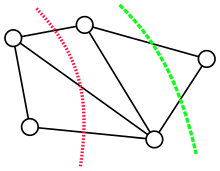
\includegraphics[width=.4\textwidth]{img/graph.png}
 \caption{Exemple de deux coupes différentes dans un graphe}
\end{figure}

Dans la figure ci-dessus, on peut voir deux possibilités de coupe différentes. Ici, puisque le graphe est non valué, la coupe rouge aura une valeur plus grande que la coupe verte.\\
Dans un graphe valué ou non, le problème du Minimum Cut Set consiste à trouver la coupe de valeur minimale dans le graphe. 